% !TeX program = xelatex
\documentclass{article}
\usepackage{kotex}
\usepackage[a4paper,left=3cm, right=3cm, top=2cm, bottom=2cm]{geometry}
\usepackage{amsmath}
\usepackage{graphicx}
\usepackage{caption}
\usepackage{setspace}
\usepackage{xcolor}
\usepackage{titlesec}
\usepackage{amssymb}
\usepackage{tcolorbox}
\usepackage{wrapfig}
\usepackage{amsthm}
\usepackage{multirow}
\usepackage{array}
\usepackage{tikz}
\usepackage{longtable}
\usepackage{pgfplots}
\pgfplotsset{compat=1.18}

\title{1.2 Gaussian Elimination}
\date{}
\author{}
\setstretch{1.3}

\titleformat{name=\section, numberless}
  {\normalfont\large\bfseries\color{blue}}
  {}
  {0pt}
  {}
\geometry{a4paper, margin=1in}

% Red subheading style (matches the textbook's red section headers)
\newcommand{\redheading}[1]{{\vspace{2mm}\noindent\Large\bfseries\color{red!55!black} #1\par}\vspace{2mm}}

\newtheoremstyle{mystyle}
  {}{}{\itshape}{}{\bfseries}{.}{.5em}{}
\theoremstyle{mystyle}

\begin{document}
\maketitle

{\itshape\color{blue!45!black}
This section develops a systematic procedure for solving linear systems: row operations that reduce the augmented matrix to a form whose solution can be read off by inspection.\par}

\redheading{Considerations in Solving Linear Systems}

Solving linear systems by hand (small systems) differs from solving them by computer (large systems, sometimes with millions of unknowns), which must also manage memory, roundoff error, and solution time -- topics of \textbf{numerical analysis}, touched on only briefly here. Even so, computer methods for large systems build on the ideas developed in this section.

\redheading{Echelon Forms}

In Example 6 of Section 1.1 we reduced an augmented matrix to
\[
\begin{bmatrix} 1&0&0&1\\ 0&1&0&2\\ 0&0&1&3\end{bmatrix}
\]
from which $x=1,y=2,z=3$ was immediate. This is a matrix in \textbf{reduced row echelon form}, meaning:
\begin{enumerate}
    \item Each nonzero row's first nonzero entry is a 1, called a \textbf{leading 1}.
    \item Zero rows are grouped at the bottom.
    \item Each leading 1 lies strictly to the right of the leading 1 in the row above.
    \item Every column containing a leading 1 is zero elsewhere.
\end{enumerate}
A matrix with only the first three properties is in \textbf{row echelon form} (reduced row echelon form is a special case).

\subsection*{EXAMPLE 1 | Row Echelon and Reduced Row Echelon Form}
Reduced row echelon form:
\[
\begin{bmatrix}1&0&0&4\\0&1&0&7\\0&0&1&-1\end{bmatrix},\quad
\begin{bmatrix}1&0&0\\0&1&0\\0&0&1\end{bmatrix},\quad
\begin{bmatrix}0&1&-2&0&1\\0&0&0&1&3\\0&0&0&0&0\\0&0&0&0&0\end{bmatrix},\quad
\begin{bmatrix}0&0\\0&0\end{bmatrix}
\]
Row echelon form but not reduced:
\[
\begin{bmatrix}1&4&-3&7\\0&1&6&2\\0&0&1&5\end{bmatrix},\quad
\begin{bmatrix}1&1&0\\0&1&0\\0&0&0\end{bmatrix},\quad
\begin{bmatrix}0&1&2&6&0\\0&0&1&-1&0\\0&0&0&0&1\end{bmatrix}
\]

\subsection*{EXAMPLE 2 | More on Row Echelon and Reduced Row Echelon Form}
Row echelon form has zeros only \emph{below} each leading 1; reduced row echelon form has zeros below \emph{and above}. With any values for the $*$'s, these are row echelon form:
\[
\begin{bmatrix}1&*&*&*\\0&1&*&*\\0&0&1&*\\0&0&0&1\end{bmatrix},\
\begin{bmatrix}1&*&*&*\\0&1&*&*\\0&0&1&*\\0&0&0&0\end{bmatrix},\
\begin{bmatrix}1&*&*&*\\0&1&*&*\\0&0&0&0\\0&0&0&0\end{bmatrix},\
\begin{bmatrix}0&1&*&*&*&*&*&*&*&*\\0&0&0&1&*&*&*&*&*&*\\0&0&0&0&1&*&*&*&*&*\\0&0&0&0&0&1&*&*&*&*\\0&0&0&0&0&0&0&0&1&*\end{bmatrix}
\]
These are reduced row echelon form:
\[
\begin{bmatrix}1&0&0&0\\0&1&0&0\\0&0&1&0\\0&0&0&1\end{bmatrix},\
\begin{bmatrix}1&0&0&*\\0&1&0&*\\0&0&1&*\\0&0&0&0\end{bmatrix},\
\begin{bmatrix}1&0&*&*\\0&1&*&*\\0&0&0&0\\0&0&0&0\end{bmatrix},\
\begin{bmatrix}0&1&*&0&0&0&*&*&0&*\\0&0&0&1&0&0&*&*&0&*\\0&0&0&0&1&0&*&*&0&*\\0&0&0&0&0&1&*&*&0&*\\0&0&0&0&0&0&0&0&1&*\end{bmatrix}
\]

Once row operations reduce an augmented matrix to \emph{reduced} row echelon form, the solution set is read off directly or converted to parametric form:

\subsection*{EXAMPLE 3 | Unique Solution}
Suppose the augmented matrix for a system in $x_1,x_2,x_3,x_4$ reduces to
\[
\begin{bmatrix}1&0&0&0&3\\0&1&0&0&-1\\0&0&1&0&0\\0&0&0&1&5\end{bmatrix}
\]
This gives $x_1=3,\ x_2=-1,\ x_3=0,\ x_4=5$ -- a unique solution, i.e.\ the 4-tuple $(3,-1,0,5)$.

\subsection*{EXAMPLE 4 | Linear Systems in Three Unknowns}
Solve the system in $x,y,z$ whose augmented matrix reduces to each of the following.
\[
(a)\ \begin{bmatrix}1&0&0&0\\0&1&2&0\\0&0&0&1\end{bmatrix}\qquad
(b)\ \begin{bmatrix}1&0&3&-1\\0&1&-4&2\\0&0&0&0\end{bmatrix}\qquad
(c)\ \begin{bmatrix}1&-5&1&4\\0&0&0&0\\0&0&0&0\end{bmatrix}
\]
\textbf{Solution (a)} The last row gives $0x+0y+0z=1$ -- inconsistent.

\textbf{Solution (b)} The last row ($0=0$) can be dropped, leaving
\[
x+3z=-1,\qquad y-4z=2
\]
Variables tied to leading 1's ($x,y$) are \textbf{leading variables}; the rest ($z$) are \textbf{free variables}. Solving for the leading variables:
\[
x=-1-3z,\qquad y=2+4z
\]
Setting $z=t$ gives the parametric equations
\[
x=-1-3t,\quad y=2+4t,\quad z=t
\]
E.g., $t=0$ gives $(-1,2,0)$; $t=1$ gives $(-4,6,1)$.

\textbf{Solution (c)} Dropping the zero rows leaves the single equation
\[
x-5y+z=4 \tag{1}
\]
-- a plane in three-dimensional space. Solving for $x$: $x=4+5y-z$; setting $y=s,\,z=t$ gives
\[
x=4+5s-t,\quad y=s,\quad z=t \tag{2}
\]

Such parametric formulas have a name:

\begin{tcolorbox}[
    colback=teal!4,
    colframe=teal!65!black,
    title=Definition 1,
    fonttitle=\bfseries,
    boxrule=0.5mm,
    arc=3mm
    ]
    For a system with infinitely many solutions, parametric equations that generate every solution by assigning numerical values to the parameters form a \textbf{general solution} of the system.
\end{tcolorbox}

Formula (2) is thus a general solution of system (c) above.

\redheading{Elimination Methods}

Once a matrix is in reduced row echelon form, solving is easy. The following step-by-step algorithm reduces \emph{any} matrix to this form, illustrated on
\[
\begin{bmatrix}0&0&-2&0&7&12\\2&4&-10&6&12&28\\2&4&-5&6&-5&-1\end{bmatrix}
\]

\noindent\textbf{Step 1.} Locate the leftmost column that is not entirely zero.
\[
\begin{bmatrix}\mathbf{0}&0&-2&0&7&12\\\mathbf{2}&4&-10&6&12&28\\\mathbf{2}&4&-5&6&-5&-1\end{bmatrix}
\quad\text{(leftmost nonzero column: column 1)}
\]

\noindent\textbf{Step 2.} If needed, interchange rows so this column's top entry is nonzero.
\[
\begin{bmatrix}2&4&-10&6&12&28\\0&0&-2&0&7&12\\2&4&-5&6&-5&-1\end{bmatrix}
\quad\text{(rows 1 and 2 interchanged)}
\]

\noindent\textbf{Step 3.} If that top entry is $a$, multiply row 1 by $1/a$ to make it a leading 1.
\[
\begin{bmatrix}1&2&-5&3&6&14\\0&0&-2&0&7&12\\2&4&-5&6&-5&-1\end{bmatrix}
\quad\text{(row 1 multiplied by $\tfrac12$)}
\]

\noindent\textbf{Step 4.} Add multiples of the top row to the rows below to zero out everything beneath the leading 1.
\[
\begin{bmatrix}1&2&-5&3&6&14\\0&0&-2&0&7&12\\0&0&5&0&-17&-29\end{bmatrix}
\quad\text{($-2\times$row 1 added to row 3)}
\]

\noindent\textbf{Step 5.} Cover the top row and repeat Steps 1--4 on the remaining submatrix, until the whole matrix is in row echelon form.
\[
\begin{bmatrix}1&2&-5&3&6&14\\0&0&1&0&-\tfrac72&-6\\0&0&5&0&-17&-29\end{bmatrix}
\quad\text{(submatrix row 1 multiplied by $-\tfrac12$)}
\]
\[
\begin{bmatrix}1&2&-5&3&6&14\\0&0&1&0&-\tfrac72&-6\\0&0&0&0&\tfrac12&1\end{bmatrix}
\quad\text{($-5\times$submatrix row 1 added to submatrix row 2)}
\]
\[
\begin{bmatrix}1&2&-5&3&6&14\\0&0&1&0&-\tfrac72&-6\\0&0&0&0&1&2\end{bmatrix}
\quad\text{(new submatrix's only row multiplied by $2$)}
\]
The matrix is now in row echelon form. One more step gives reduced row echelon form.

\noindent\textbf{Step 6.} Working upward from the last nonzero row, add multiples of each row to the rows above to zero out everything above the leading 1's.
\[
\begin{bmatrix}1&2&-5&3&6&14\\0&0&1&0&0&1\\0&0&0&0&1&2\end{bmatrix}
\quad\text{($\tfrac72\times$row 3 added to row 2)}
\]
\[
\begin{bmatrix}1&2&-5&3&0&2\\0&0&1&0&0&1\\0&0&0&0&1&2\end{bmatrix}
\quad\text{($-6\times$row 3 added to row 1)}
\]
\[
\begin{bmatrix}1&2&0&3&0&7\\0&0&1&0&0&1\\0&0&0&0&1&2\end{bmatrix}
\quad\text{($5\times$row 2 added to row 1)}
\]
This last matrix is in reduced row echelon form.

This algorithm is \textbf{Gauss--Jordan elimination}: a \textbf{forward phase} (zeros below the leading 1's) followed by a \textbf{backward phase} (zeros above). Using only the forward phase yields a row echelon form and is called \textbf{Gaussian elimination} -- as obtained above at the end of Step 5.

\subsection*{EXAMPLE 5 | Gauss--Jordan Elimination}
Solve by Gauss--Jordan elimination.
\[
\begin{aligned}
x_1+3x_2-2x_3\qquad\qquad+2x_5\qquad\qquad&=0\\
2x_1+6x_2-5x_3-2x_4+4x_5-3x_6&=-1\\
5x_3+10x_4\qquad\qquad+15x_6&=5\\
2x_1+6x_2\qquad\qquad+8x_4+4x_5+18x_6&=6
\end{aligned}
\]
\textbf{SOLUTION:} The augmented matrix is
\[
\begin{bmatrix}1&3&-2&0&2&0&0\\2&6&-5&-2&4&-3&-1\\0&0&5&10&0&15&5\\2&6&0&8&4&18&6\end{bmatrix}
\]
Add $-2\times$row 1 to rows 2 and 4:
\[
\begin{bmatrix}1&3&-2&0&2&0&0\\0&0&-1&-2&0&-3&-1\\0&0&5&10&0&15&5\\0&0&4&8&0&18&6\end{bmatrix}
\]
Multiply row 2 by $-1$, then add $-5\times$(new row 2) to row 3 and $-4\times$(new row 2) to row 4:
\[
\begin{bmatrix}1&3&-2&0&2&0&0\\0&0&1&2&0&3&1\\0&0&0&0&0&0&0\\0&0&0&0&0&6&2\end{bmatrix}
\]
Interchange rows 3 and 4, then multiply the new row 3 by $\tfrac16$ -- the row echelon form:
\[
\begin{bmatrix}1&3&-2&0&2&0&0\\0&0&1&2&0&3&1\\0&0&0&0&0&1&\tfrac13\\0&0&0&0&0&0&0\end{bmatrix}
\]
Forward phase complete. Add $-3\times$row 3 to row 2, then $2\times$(new row 2) to row 1 -- the reduced row echelon form:
\[
\begin{bmatrix}1&3&0&4&2&0&0\\0&0&1&2&0&0&0\\0&0&0&0&0&1&\tfrac13\\0&0&0&0&0&0&0\end{bmatrix}
\]
Backward phase complete; the corresponding system is
\[
x_1+3x_2\qquad\ +4x_4+2x_5\qquad=0,\qquad x_3+2x_4\qquad=0,\qquad x_6=\tfrac13 \tag{3}
\]
Solving for the leading variables:
\[
x_1=-3x_2-4x_4-2x_5,\qquad x_3=-2x_4,\qquad x_6=\tfrac13
\]
Assigning the free variables $x_2,x_4,x_5$ the parameters $r,s,t$ gives the general solution:
\[
x_1=-3r-4s-2t,\quad x_2=r,\quad x_3=-2s,\quad x_4=s,\quad x_5=t,\quad x_6=\tfrac13
\]

\redheading{Homogeneous Linear Systems}

A linear system is \textbf{homogeneous} if all constant terms are zero:
\[
\begin{aligned}
a_{11}x_1+a_{12}x_2+\cdots+a_{1n}x_n&=0\\
a_{21}x_1+a_{22}x_2+\cdots+a_{2n}x_n&=0\\
&\ \ \vdots\\
a_{m1}x_1+a_{m2}x_2+\cdots+a_{mn}x_n&=0
\end{aligned}
\]
Every homogeneous system is consistent, since $x_1=\cdots=x_n=0$ (the \textbf{trivial solution}) always works; any other solution is \textbf{nontrivial}.

So only two outcomes are possible:
\begin{itemize}
    \item The system has only the trivial solution.
    \item The system has infinitely many solutions in addition to the trivial solution.
\end{itemize}
For two homogeneous equations in two unknowns,
\[
a_1x+b_1y=0\ [a_1,b_1\text{ not both zero}],\qquad a_2x+b_2y=0\ [a_2,b_2\text{ not both zero}],
\]
both graphs are lines through the origin, and the trivial solution is their common point there (\textbf{Figure 1.2.1}).

\begin{figure}[h]
\centering
\begin{tabular}{cc}
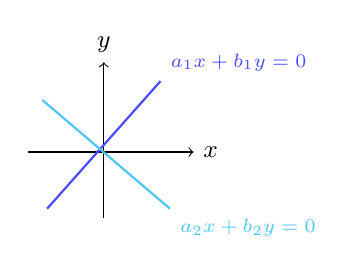
\begin{tikzpicture}[scale=0.6]
 \draw[->] (-1.6,0)--(1.9,0) node[right]{\small$x$};
 \draw[->] (0,-1.4)--(0,1.9) node[above]{\small$y$};
 \draw[blue!70,thick] (-1.2,-1.2)--(1.2,1.5) node[above right]{\scriptsize$a_1x+b_1y=0$};
 \draw[cyan!70,thick] (-1.3,1.1)--(1.4,-1.2) node[below right]{\scriptsize$a_2x+b_2y=0$};
\end{tikzpicture}
&
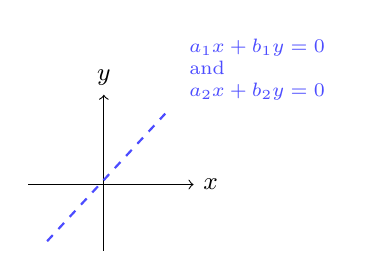
\begin{tikzpicture}[scale=0.6]
 \draw[->] (-1.6,0)--(1.9,0) node[right]{\small$x$};
 \draw[->] (0,-1.4)--(0,1.9) node[above]{\small$y$};
 \draw[blue!70,thick,dashed] (-1.2,-1.2)--(1.3,1.5) node[above right]{\scriptsize$\begin{array}{l}a_1x+b_1y=0\\ \text{and}\\ a_2x+b_2y=0\end{array}$};
\end{tikzpicture}
\\
\fbox{\small Only the trivial solution} & \fbox{\small Infinitely many solutions}
\end{tabular}
\caption*{\textbf{FIGURE 1.2.1}}
\end{figure}

One case guarantees nontrivial solutions: more unknowns than equations. Consider four equations in six unknowns.

\subsection*{EXAMPLE 6 | A Homogeneous System}
Use Gauss--Jordan elimination to solve the homogeneous linear system
\[
\begin{aligned}
x_1+3x_2-2x_3\qquad\qquad+2x_5\qquad\qquad&=0\\
2x_1+6x_2-5x_3-2x_4+4x_5-3x_6&=0\\
5x_3+10x_4\qquad\qquad+15x_6&=0\\
2x_1+6x_2\qquad\qquad+8x_4+4x_5+18x_6&=0
\end{aligned} \tag{4}
\]
\textbf{SOLUTION:} This is Example 5's system with all right-hand sides set to zero, so its reduced row echelon form matches Example 5's except the last column is all zeros (row operations never change a zero column):
\[
\begin{bmatrix}1&3&0&4&2&0&0\\0&0&1&2&0&0&0\\0&0&0&0&0&1&0\\0&0&0&0&0&0&0\end{bmatrix}
\]
The corresponding system is
\[
x_1+3x_2\qquad+4x_4+2x_5=0,\qquad x_3+2x_4=0,\qquad x_6=0
\]
giving $x_1=-3x_2-4x_4-2x_5,\ x_3=-2x_4,\ x_6=0$. With $x_2,x_4,x_5=r,s,t$, the parametric solution is
\[
x_1=-3r-4s-2t,\quad x_2=r,\quad x_3=-2s,\quad x_4=s,\quad x_5=t,\quad x_6=0
\]
(The trivial solution is $r=s=t=0$.)

\redheading{Free Variables in Homogeneous Linear Systems}

Example 6 illustrates two points about homogeneous systems:
\begin{enumerate}
    \item Row operations never change a zero column, so the reduced row echelon form of a homogeneous system's augmented matrix keeps its zero last column -- the reduced system stays homogeneous.
    \item A zero row corresponds to $0=0$, which imposes no condition and can be dropped -- so the reduced system may have fewer equations than the original.
\end{enumerate}

In general, for $n$ unknowns and $r$ nonzero rows in the reduced row echelon form, there are $r$ leading variables and $n-r$ free variables.

\begin{tcolorbox}[colback=red!4, colframe=red!60!black, title=Theorem 1.2.1 -- Free Variable Theorem for Homogeneous Systems, boxrule=0.5mm, arc=3mm]
If a homogeneous linear system has $n$ unknowns, and if the reduced row echelon form of its augmented matrix has $r$ nonzero rows, then the system has $n-r$ free variables.
\end{tcolorbox}

If $m<n$ (fewer equations than unknowns), then $r<n$, so there is at least one free variable -- hence infinitely many solutions:

\begin{tcolorbox}[colback=red!4, colframe=red!60!black, title=Theorem 1.2.2, boxrule=0.5mm, arc=3mm]
A homogeneous linear system with more unknowns than equations has infinitely many solutions.
\end{tcolorbox}

So Example 6's system (4 equations, 6 unknowns) was guaranteed to have infinitely many solutions.

\redheading{Gaussian Elimination and Back-Substitution}

Gauss--Jordan elimination suits hand computation; for large computer-solved systems, Gaussian elimination (row echelon form) plus \textbf{back-substitution} is typically more efficient:

\subsection*{EXAMPLE 7 | Example 5 Solved by Back-Substitution}
From Example 5's row echelon form
\[
\begin{bmatrix}1&3&-2&0&2&0&0\\0&0&1&2&0&3&1\\0&0&0&0&0&1&\tfrac13\\0&0&0&0&0&0&0\end{bmatrix}
\]
solve the corresponding system
\[
x_1+3x_2-2x_3\qquad\ +2x_5\qquad=0,\qquad x_3+2x_4\qquad+3x_6=1,\qquad x_6=\tfrac13
\]
as follows:

\noindent\textbf{Step 1.} Solve the equations for the leading variables.
\[
x_1=-3x_2+2x_3-2x_5,\qquad x_3=1-2x_4-3x_6,\qquad x_6=\tfrac13
\]

\noindent\textbf{Step 2.} Starting from the bottom, substitute each equation into those above it.

Substituting $x_6=\tfrac13$ into the second equation:
\[
x_1=-3x_2+2x_3-2x_5,\qquad x_3=-2x_4,\qquad x_6=\tfrac13
\]
Substituting $x_3=-2x_4$ into the first equation:
\[
x_1=-3x_2-4x_4-2x_5,\qquad x_3=-2x_4,\qquad x_6=\tfrac13
\]

\noindent\textbf{Step 3.} Assign arbitrary values to the free variables, if any.

Assigning $x_2,x_4,x_5=r,s,t$ gives the general solution
\[
x_1=-3r-4s-2t,\quad x_2=r,\quad x_3=-2s,\quad x_4=s,\quad x_5=t,\quad x_6=\tfrac13
\]
matching Example 5.

\subsection*{EXAMPLE 8 | Existence and Uniqueness of Solutions}
Each matrix below is a row-echelon (not reduced) augmented matrix for a system in $x_1,x_2,x_3,x_4$. Discuss existence and uniqueness of solutions.
\[
(a)\ \begin{bmatrix}1&-3&7&2&5\\0&1&2&-4&1\\0&0&1&6&9\\0&0&0&0&1\end{bmatrix}\qquad
(b)\ \begin{bmatrix}1&-3&7&2&5\\0&1&2&-4&1\\0&0&1&6&9\\0&0&0&0&0\end{bmatrix}
\]
\[
(c)\ \begin{bmatrix}1&-3&7&2&5\\0&1&2&-4&1\\0&0&1&6&9\\0&0&0&1&0\end{bmatrix}
\]
\textbf{Solution (a)} Last row: $0x_1+0x_2+0x_3+0x_4=1$ -- inconsistent.

\textbf{Solution (b)} Last row: $0=0$, no effect. $x_1,x_2,x_3$ are leading variables, $x_4$ is free -- infinitely many solutions.

\textbf{Solution (c)} Last row gives $x_4=0$; back-substituting into $x_3+6x_4=9$ gives $x_3=9$, and continuing upward pins down $x_2$ then $x_1$ uniquely -- a unique solution.

\redheading{Some Facts About Echelon Forms}

Three facts worth knowing (not proved here):
\begin{enumerate}
    \item Every matrix has a unique reduced row echelon form, regardless of which sequence of row operations is used.
    \item Row echelon forms, however, are not unique -- different operation sequences can give different results.
    \item Still, every row echelon form of a matrix $A$ has the same number of zero rows and the same leading-1 positions, called the \textbf{pivot positions} of $A$; the columns/rows containing them are the \textbf{pivot columns}/\textbf{pivot rows}, and a nonzero entry in a pivot position is a \textbf{pivot} of $A$.
\end{enumerate}

\subsection*{EXAMPLE 9 | Pivot Positions and Columns}
Earlier we reduced
\[
A=\begin{bmatrix}0&0&-2&0&7&12\\2&4&-10&6&12&28\\2&4&-5&6&-5&-1\end{bmatrix}
\quad\text{to}\quad
\begin{bmatrix}1&2&-5&3&6&14\\0&0&1&0&-\tfrac72&-6\\0&0&0&0&1&2\end{bmatrix}
\]
The leading 1's sit at (row 1, col 1), (row 2, col 3), (row 3, col 5) -- the pivot positions. So the pivot columns are 1, 3, 5; the pivot rows are 1, 2, 3; and the pivots are the entries there.

\redheading{Roundoff Error and Instability}

Theory and practice can diverge: computers approximate numbers, introducing \textbf{roundoff} error that, uncontrolled, can make an algorithm \textbf{unstable}. Since Gauss--Jordan elimination takes roughly 50\% more operations than Gaussian elimination on large systems, most computer algorithms use the latter.

\section*{Exercise Set 1.2}
\begin{enumerate}
    \item[1.] Classify each matrix as row echelon form, reduced row echelon form, both, or neither.\\
    (a) $\begin{bmatrix}1&0&0\\0&1&0\\0&0&1\end{bmatrix}$
    (b) $\begin{bmatrix}1&0&0\\0&1&0\\0&0&0\end{bmatrix}$
    (c) $\begin{bmatrix}0&1&0\\0&0&1\\0&0&0\end{bmatrix}$\\[2mm]
    (d) $\begin{bmatrix}1&0&3&1\\0&1&2&4\end{bmatrix}$
    (e) $\begin{bmatrix}1&2&0&3&0\\0&0&1&1&0\\0&0&0&0&1\\0&0&0&0&0\end{bmatrix}$\\[2mm]
    (f) $\begin{bmatrix}0&0\\0&0\\0&0\end{bmatrix}$
    (g) $\begin{bmatrix}1&-7&5&5\\0&1&3&2\end{bmatrix}$

    \item[3.] Each augmented matrix below is a row echelon form reached by row operations. Identify its pivot rows/columns and solve the system.\\
    (a) $\begin{bmatrix}1&-3&4&7\\0&1&2&2\\0&0&1&5\end{bmatrix}$
    (b) $\begin{bmatrix}1&0&8&-5&6\\0&1&4&-9&3\\0&0&1&1&2\end{bmatrix}$\\[2mm]
    (c) $\begin{bmatrix}1&7&-2&0&-8&-3\\0&0&1&1&6&5\\0&0&0&1&3&9\\0&0&0&0&0&0\end{bmatrix}$
    (d) $\begin{bmatrix}1&-3&7&1\\0&1&4&0\\0&0&0&1\end{bmatrix}$

    \item[5.] Solve by Gaussian elimination.\\
    $x_1+x_2+2x_3=8,\quad -x_1-2x_2+3x_3=1,\quad 3x_1-7x_2+4x_3=10$

    \item[7.] Solve by Gaussian elimination.\\
    $x-y+2z-w=-1,\quad 2x+y-2z-2w=-2,\quad -x+2y-4z+w=1,\quad 3x-3w=-3$

    \item[9.] Solve Exercise 5 by Gauss--Jordan elimination.

    \item[11.] Solve Exercise 7 by Gauss--Jordan elimination.

    \item[13.] Determine by inspection (no pencil and paper) whether the homogeneous system has nontrivial solutions.\\
    $2x_1-3x_2+4x_3-x_4=0,\quad 7x_1+x_2-8x_3+9x_4=0,\quad 2x_1+8x_2+x_3-x_4=0$

    \item[15.] Solve by any method.\\
    $2x_1+x_2+3x_3=0,\quad x_1+2x_2=0,\quad x_2+x_3=0$

    \item[17.] Solve by any method.\\
    $3x_1+x_2+x_3+x_4=0,\quad 5x_1-x_2+x_3-x_4=0$

    \item[21.] Solve by any method.\\
    $2I_1-I_2+3I_3+4I_4=9,\quad I_1-2I_3+7I_4=11,\quad 3I_1-3I_2+I_3+5I_4=8,\quad 2I_1+I_2+4I_3+4I_4=10$

    \item[23.] Each augmented matrix below has unspecified entries $*$. Determine whether the system is consistent and, if so, whether the solution is unique -- answer ``inconclusive'' if there isn't enough information.\\
    (a) $\begin{bmatrix}1&*&*&*\\0&1&*&*\\0&0&1&*\end{bmatrix}$
    (b) $\begin{bmatrix}1&*&*&*\\0&1&*&*\\0&0&0&0\end{bmatrix}$
    (c) $\begin{bmatrix}1&*&*&*\\0&1&*&*\\0&0&0&1\end{bmatrix}$
    (d) $\begin{bmatrix}1&*&*&*\\0&0&*&0\\0&0&1&*\end{bmatrix}$

    \item[25.] Determine the values of $a$ for which the system has no solution, exactly one solution, or infinitely many solutions.\\
    $x+2y-3z=4,\quad 3x-y+5z=2,\quad 4x+y+(a^2-14)z=a+2$

    \item[27.] What condition, if any, must $a$, $b$, $c$ satisfy for the system to be consistent?\\
    $x+3y-z=a,\quad x+y+2z=b,\quad 2y-3z=c$

    \item[31.] Find two different row echelon forms of
    \[
    \begin{bmatrix}1&3\\2&7\end{bmatrix}
    \]
    -- showing that row echelon forms need not be unique.

    \item[32.] Reduce
    \[
    \begin{bmatrix}2&1&3\\0&-2&-29\\3&4&5\end{bmatrix}
    \]
    to reduced row echelon form without introducing fractions at any intermediate stage.

    \item[33.] Show that the following nonlinear system has 18 solutions for $0\le\alpha,\beta,\gamma\le2\pi$.
    \[
    \sin\alpha+2\cos\beta+3\tan\gamma=0,\qquad 2\sin\alpha+5\cos\beta+3\tan\gamma=0,\qquad -\sin\alpha-5\cos\beta+5\tan\gamma=0
    \]
    [\emph{Hint:} substitute $x=\sin\alpha$, $y=\cos\beta$, $z=\tan\gamma$.]

    \item[35.] Solve the following nonlinear system for $x,y,z$.
    \[
    x^2+y^2+z^2=6,\qquad x^2-y^2+2z^2=2,\qquad 2x^2+y^2-z^2=3
    \]
    [\emph{Hint:} substitute $X=x^2$, $Y=y^2$, $Z=z^2$.]

    \item[37.] Find $a,b,c,d$ so that the curve shown is the graph of $y=ax^3+bx^2+cx+d$.
    \begin{figure}[h]
    \centering
    \begin{tikzpicture}[scale=0.65]
    \begin{scope}
    \clip (-2.5,-6.1) rectangle (6.7,6.6);
    \draw[->] (-2.4,0)--(6.6,0) node[right]{\small$x$};
    \draw[->] (0,-6)--(0,6.5) node[above]{\small$y$};
    \draw[blue!70,thick,domain=-2.2:6.35,samples=150] plot(\x,{(\x*\x*\x-6*\x*\x+2*\x+10)/6});
    \draw (-0.08,3.333)--(0.08,3.333) node[right]{\scriptsize$20$};
    \draw (-0.08,-3.333)--(0.08,-3.333) node[right]{\scriptsize$-20$};
    \filldraw[black] (0,1.667) circle (1pt) node[above right]{\scriptsize$(0,10)$};
    \filldraw[black] (1,1.167) circle (1pt) node[above right]{\scriptsize$(1,7)$};
    \filldraw[black] (3,-1.833) circle (1pt) node[below]{\scriptsize$(3,-11)$};
    \filldraw[black] (4,-2.333) circle (1pt) node[below right]{\scriptsize$(4,-14)$};
    \node at (-2.1,0.35) {\scriptsize$-2$};
    \node at (6.15,0.35) {\scriptsize$6$};
    \end{scope}
    \end{tikzpicture}
    \caption*{\textbf{FIGURE Ex-37}}
    \end{figure}

    \item[39.] If the linear system
    \[
    a_1x+b_1y+c_1z=0,\qquad a_2x-b_2y+c_2z=0,\qquad a_3x+b_3y-c_3z=0
    \]
    has only the trivial solution, what can be said about the solutions of
    \[
    a_1x+b_1y+c_1z=3,\qquad a_2x-b_2y+c_2z=7,\qquad a_3x+b_3y-c_3z=11\ ?
    \]

    \item[40.] (a) If $A$ has three rows and five columns, what is the maximum possible number of leading 1's in its reduced row echelon form?\\
    (b) If $B$ has three rows and six columns, what is the maximum possible number of parameters in the general solution of the system with augmented matrix $B$?\\
    (c) If $C$ has five rows and three columns, what is the minimum possible number of zero rows in any row echelon form of $C$?

    \item[41.] Describe all possible reduced row echelon forms of\\
    (a) $\begin{bmatrix}a&b&c\\d&e&f\\g&h&i\end{bmatrix}$\qquad
    (b) $\begin{bmatrix}a&b&c&d\\e&f&g&h\\i&j&k&l\\m&n&p&q\end{bmatrix}$
\end{enumerate}

\end{document}
